\section{Evaluation}
\label{sec:eval}
% 评估

This section evaluates \lang, the hardware-idiom instantiation of \tool.
% 本节评估 \lang，\tool 的硬件习语实例。
\tool provides the extension interface, while \lang provides the concrete operations used in our experiments.
% \tool 提供扩展接口，而 \lang 提供我们实验中使用的具体操作。
\lang complements bytecode optimizers~\cite{xu2021synthesizing,mao2024merlin,zhu2025epso}, which cannot emit native instructions that the eBPF instruction set lacks.
% \lang 与字节码优化器互补，后者无法发射 eBPF 指令集缺少的本地指令。
We use two workload classes.
% 我们使用两类工作负载。
First, we reuse the 27 microbenchmarks from \S\ref{sec:characterization} to isolate instruction-selection effects.
% 首先，我们重用来自特征分析的 27 个纯字节码微基准测试来隔离指令选择效果。
Second, we use production packet-processing applications to test whether those effects carry over to real deployments.
% 其次，我们使用生产环境的包处理应用，测试这些效果能否延续到真实部署中。
We answer four questions:
% 我们回答四个问题：

\begin{itemize}
\item \textbf{RQ1:} How much does \lang speed up microbenchmarks on x86-64 and ARM64?
% RQ1：\lang 在 x86-64 和 ARM64 上使微基准测试加速多少？
\item \textbf{RQ2:} How does \lang perform on production applications?
% RQ2：\lang 在生产应用上的表现如何？
\item \textbf{RQ3:} How sensitive is \lang to its operation-selection policy?
% RQ3：\lang 对操作选择策略的敏感度如何？
\item \textbf{RQ4:} How does \tool compare with an in-kernel native upper bound?
% RQ4：\tool 与内核内原生上界相比如何？
\end{itemize}

\paragraph{Evaluation environment.}
% \paragraph{评估环境。}
\note{format inconsistent}
We use two evaluation platforms.
% 我们使用两个评估平台。
The x86-64 experiments run in a KVM virtual machine with 8 vCPUs and 64\,GB RAM on an Intel Core Ultra 9 285K host, using Linux 7.0.0-rc2+.
% x86-64 实验在 Intel Core Ultra 9 285K 主机上的 KVM 虚拟机中运行，配置 8 个 vCPU 和 64 GB RAM，使用 Linux 7.0.0-rc2+。
The ARM64 experiments run on an AWS t4g.small instance (2 vCPUs, 2\,GiB RAM, AWS Graviton2), using a \lang-enabled Linux 7.0.0-rc2+ build.
% ARM64 实验在 AWS t4g.small 实例（2 个 vCPU，2 GiB RAM，AWS Graviton2）上运行，使用启用 \lang 的 Linux 7.0.0-rc2+ 构建。
These platforms cover both the microbenchmark suite and the production-application experiments.
% 这些平台涵盖微基准测试套件和生产应用实验。
For matched application comparisons, the original and \lang runs use the same kernel image and differ only in whether the loaded program uses \lang operations and in the \lang policy.
% 对于匹配的应用比较，原版和 \lang 运行使用相同的内核镜像，仅在加载的程序是否使用 \lang 操作以及 \lang 策略上不同。

\paragraph{Measurement conventions.}
% \paragraph{测量约定。}
Unless otherwise stated, each experiment uses three measured runs and reports the median.
% 除非另有说明，每个实验使用三次测量运行并报告中位数。
Execution-time and throughput ratios are normalized to the original kernel JIT, so values above 1$\times$ indicate faster execution or higher throughput.
% 执行时间和吞吐量比率归一化到原版内核 JIT，因此高于 1 倍的值表示更快的执行或更高的吞吐量。
BPF cost is the average run time of a BPF program per invocation, as reported by the kernel. BPF-cost ratios divide the \lang cost by the original cost, so values below 1$\times$ indicate lower cost.
% BPF 成本是内核报告的 BPF 程序每次调用的平均运行时间；BPF 成本比率是 \lang 成本除以原版成本，因此低于 1 倍的值表示成本更低。
We compute it from the kernel's per-program runtime statistics as the change in total run time divided by the change in run count, match programs across the two runs by name, type, and order of appearance, and drop programs that run fewer than 100 times in either run.
% 我们根据内核的逐程序运行时统计计算它：总运行时间的变化除以运行次数的变化；按名称、类型和出现顺序在两次运行之间匹配程序，并丢弃在任一次运行中运行少于 100 次的程序。



\subsection{RQ1: Microbenchmarks on x86-64 and ARM64}
\label{subsec:micro_benchmark}

\begin{figure*}[t]
\centering

\begin{subfigure}[t]{\textwidth}
\centering
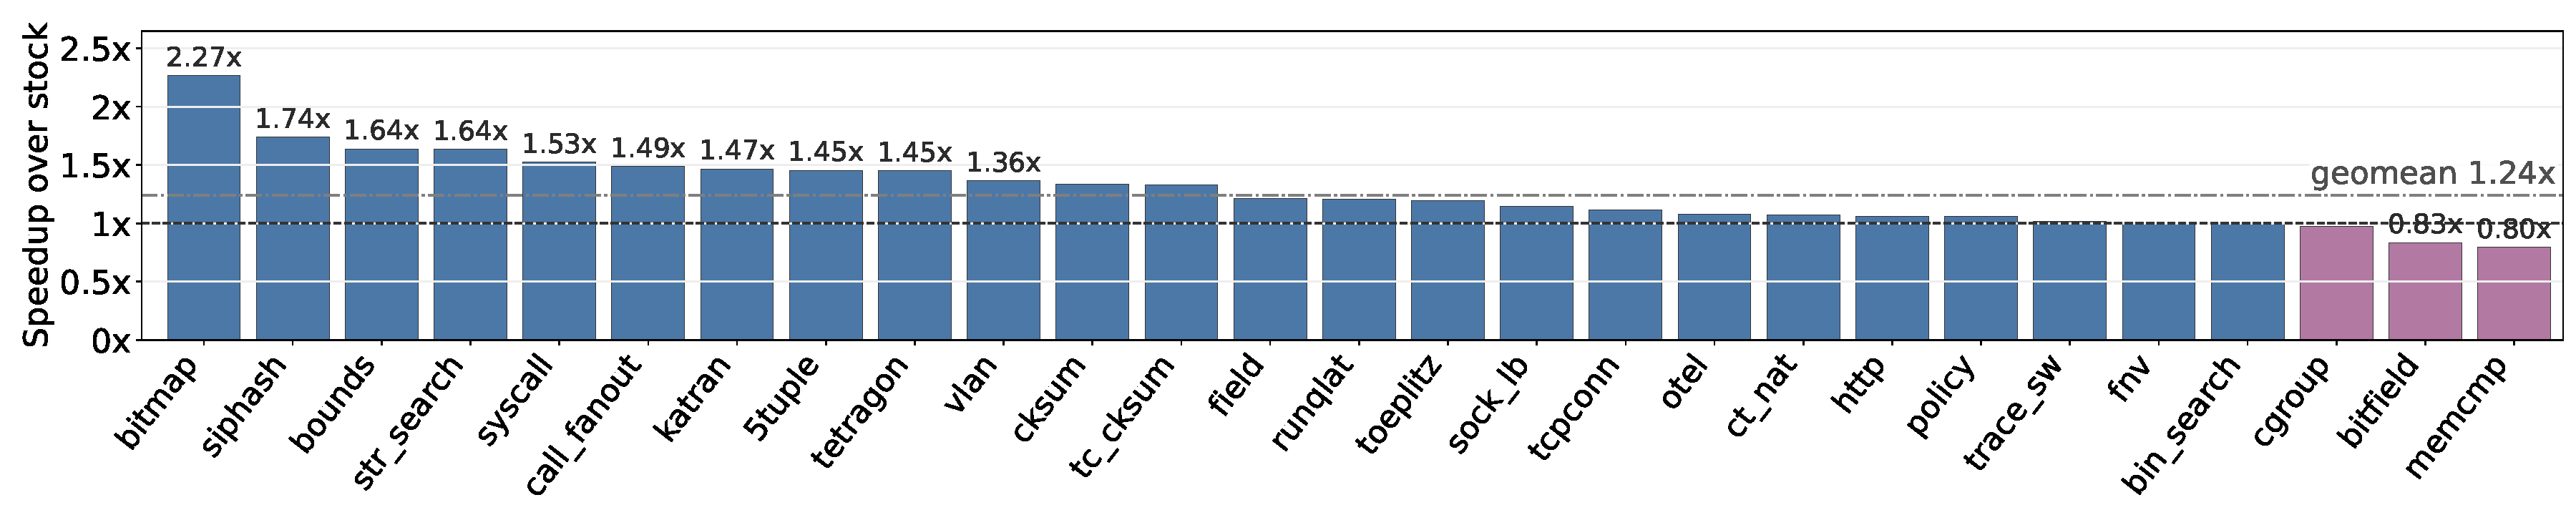
\includegraphics[width=\textwidth]{figures/sec-6-x86-kinsn-micro-best-raw-27-20260608.pdf}
\caption{x86-64.}
\label{fig:eval-kinsn-micro-x86}
\end{subfigure}

\vspace{0.2em}

\begin{subfigure}[t]{\textwidth}
\centering
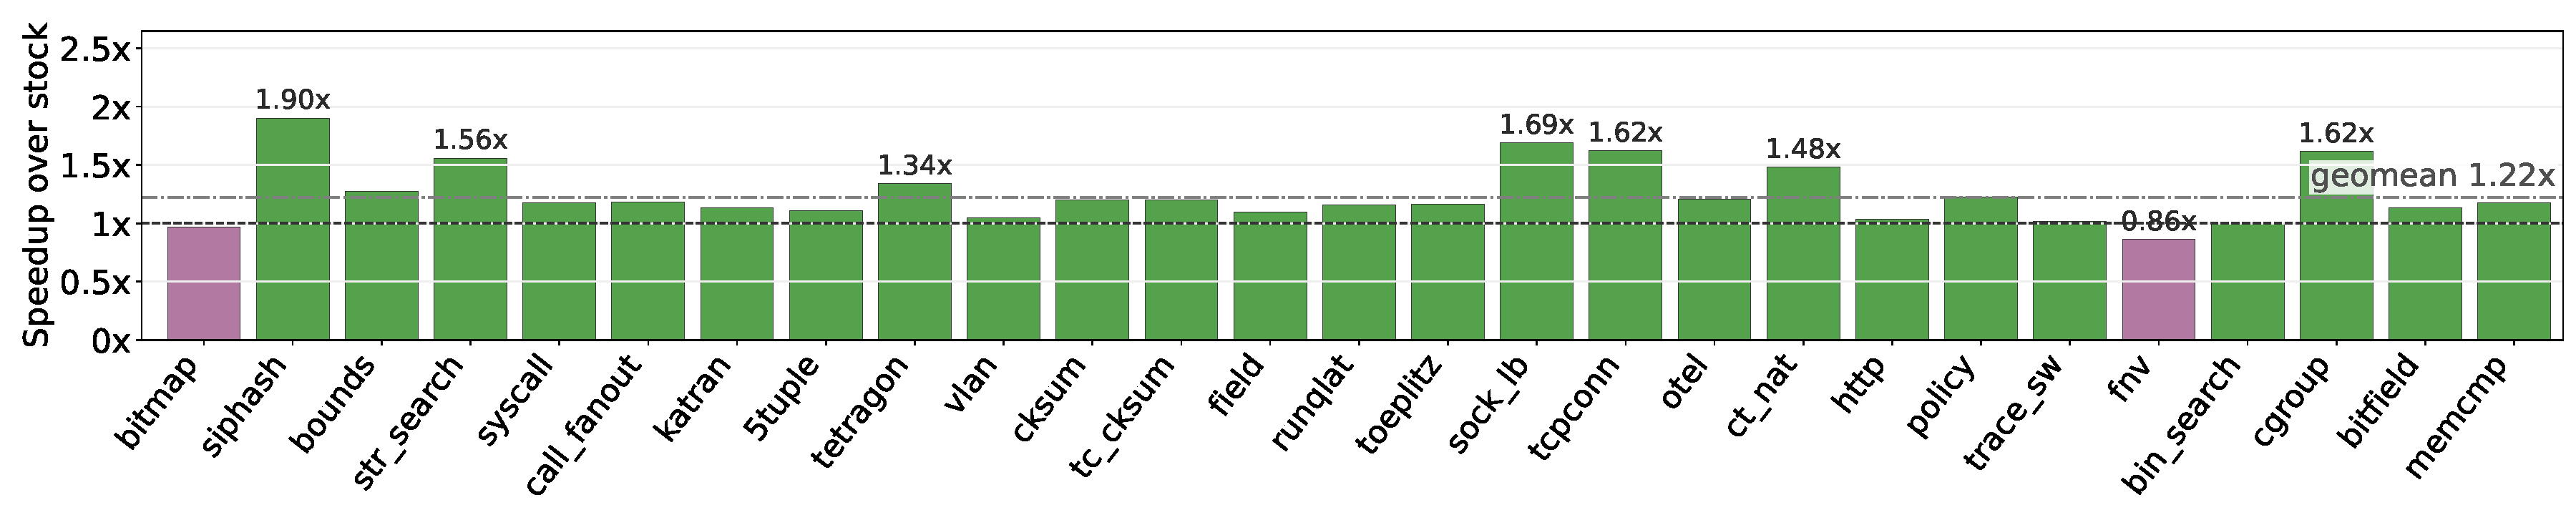
\includegraphics[width=\textwidth]{figures/sec-6-arm64-kinsn-micro-rejit-27-20260608.pdf}
\caption{ARM64.}
\label{fig:eval-kinsn-micro-arm64}
\end{subfigure}

\caption{Microbenchmark speedup in median execution time over the original eBPF JIT, with 100,000 iterations per sample. Panel~(b) covers the 27 benchmarks with rewritten \lang{} sites. Red lines mark the geometric mean speedup.}
\label{fig:eval-kinsn-micro}
\end{figure*}


RQ1 evaluates how much \lang's hardware-idiom operations speed up the microbenchmarks.
% RQ1 评估 \lang 的硬件习语操作使微基准加速多少。
\lang reduces the size of the code the kernel JIT generates on both architectures: relative to the original kernel JIT, the code shrinks to 0.772$\times$ on x86-64 and 0.879$\times$ on ARM64, geometric mean reductions of 22.8\% and 12.1\%.
% \lang 在两种架构上都减小了内核 JIT 生成的代码：相对原版内核 JIT，代码在 x86-64 上缩小到 0.772 倍，在 ARM64 上缩小到 0.879 倍，几何平均分别减少 22.8\% 和 12.1\%。

Figure~\ref{fig:eval-kinsn-micro} reports execution time.
% 图报告了执行时间。
On x86-64, \lang achieves a 1.242$\times$ geometric mean speedup over the original kernel JIT, reducing execution time by 19.47\%.
% 在 x86-64 上，\lang 相对原版内核 JIT 取得 1.242 倍的几何平均加速，执行时间减少 19.47\%。
On ARM64, \lang rewrites all 308 matched \emph{sites}, the places where the recognizer replaces an idiom with an extended instruction, and achieves a 1.222$\times$ geometric mean speedup over the 27 benchmarks, reducing execution time by 18.17\%.
% 在 ARM64 上，\lang 改写了全部 308 个匹配的\emph{站点}（即识别器用扩展指令替换习语的位置），在 27 个基准上取得 1.222 倍的几何平均加速，执行时间减少 18.17\%。
On both architectures, every benchmark produces the same output as under the original kernel JIT.
% 在两种架构上，每个基准的输出都与原版内核 JIT 下相同。
On x86-64, the 1.242$\times$ speedup recovers 42\% of the characterization's 1.57$\times$ gap to native code $((1.242{-}1)/(1.57{-}1))$.
% 在 x86-64 上，1.242 倍的加速追回了特征分析中与本地代码 1.57 倍差距的 42\%。



The per-benchmark results suggest different sources of benefit on the two architectures.
% 逐基准的结果表明两种架构上的收益来源不同。
On x86-64, speedups follow code-size reduction more closely, consistent with \lang replacing the original JIT's conservative instruction sequences and executing fewer instructions.
% 在 x86-64 上，加速与代码大小的减少更为相关，这与 \lang 替换原版 JIT 的保守指令序列、执行更少指令一致。
On ARM64, code size explains less: the largest gains appear where the recognizer rewrites rotates, bit extracts, and packet-field loads.
% 在 ARM64 上，代码大小的解释力较弱：最大的收益出现在识别器改写旋转、位提取和包字段加载的地方。
For example, \texttt{siphash\_rotate64\_\allowbreak mixer}, whose rewritten sites mostly emit extract instructions, reaches a 1.902$\times$ speedup on ARM64, and networking microbenchmarks such as Cilium socket load balancing, BCC TCP tuple filtering, and Cilium CT/NAT tuple rewriting reach 1.691$\times$, 1.624$\times$, and 1.482$\times$.
% 例如，改写站点大多发射提取指令的 siphash\_rotate64\_mixer 在 ARM64 上达到 1.902 倍加速；Cilium 套接字负载均衡、BCC TCP 元组过滤和 Cilium CT/NAT 元组改写等网络微基准分别达到 1.691、1.624 和 1.482 倍。
\lang is therefore not merely a code-size optimization. Its effect depends on the architecture, the original JIT's code, the operations used, and whether the rewritten sites lie on hot paths.
% 因此 \lang 不只是代码大小优化；其效果取决于架构、原版 JIT 的代码、所用的操作，以及改写站点是否位于热路径上。

The regressions also show the current limits of the recognizer.
% 性能回退也显示了识别器目前的局限。
\texttt{bpftrace\_comm\_key\_fnv\_hash} slows to 0.862$\times$ on ARM64, and \texttt{bitmap\_popcount\_scan} slows to 0.966$\times$ even though \lang rewrites some of its sites.
% bpftrace\_comm\_key\_fnv\_hash 在 ARM64 上降到 0.862 倍，bitmap\_popcount\_scan 尽管有站点被 \lang 改写，也降到 0.966 倍。
These cases indicate that \lang is not uniformly beneficial and that operations should be enabled selectively, for example with a lightweight cost model, rather than at every matched site.
% 这些情况说明 \lang 并非处处有益，应当有选择地启用操作（例如借助轻量的代价模型），而不是在每个匹配站点都启用。

\noindent\textbf{Load-time overhead.}
% \noindent\textbf{加载时开销。}
Replacing extended instructions before verification and restoring them afterward adds two linear passes over the program.
% 在验证前替换扩展指令、验证后恢复，给程序增加两遍线性扫描。
Across all 62 microbenchmarks on x86-64, the kernel's load time, which covers verification and JIT compilation, is 0.99$\times$ that of the original kernel in geometric mean, so the overhead is not measurable.
% 在 x86-64 上的全部 62 个微基准中，内核加载时间（包括验证和 JIT 编译）的几何平均是原版内核的 0.99 倍，开销无法测出。
For programs with \lang sites, the end-to-end compile time, including the userspace recognizer, increases by 1.4--2.4$\times$ but stays below a millisecond.
% 对于含有 \lang 站点的程序，端到端编译时间（包括用户空间识别器）增加 1.4--2.4 倍，但仍低于一毫秒。



\subsection{RQ2: Real Packet-Processing Applications}
\label{subsec:corpus_application}

RQ2 evaluates the same operations on production packet-processing applications.
% RQ2 在生产环境的包处理应用上评估同样的操作。
Microbenchmarks isolate individual instruction patterns, but packet-processing applications combine those patterns with maps, helper calls, tail calls, and application-specific datapath structure.
% 微基准隔离了单个指令模式，而包处理应用把这些模式与 map、辅助函数调用、尾调用以及应用特有的数据路径结构结合在一起。
We therefore evaluate \lang on two real eBPF packet-processing applications: Cilium and Katran.
% 因此我们在两个真实的 eBPF 包处理应用 Cilium 和 Katran 上评估 \lang。
Cilium represents a large tail-call-heavy Kubernetes datapath, while Katran represents a compact high-rate XDP load balancer with a hot directly attached program.
% Cilium 代表大量使用尾调用的大型 Kubernetes 数据路径，Katran 代表一个紧凑、高速率、直接挂载热程序的 XDP 负载均衡器。
We measure end-to-end datapath throughput with BPF runtime statistics disabled to avoid measurement overhead.
% 我们在关闭 BPF 运行时统计的情况下测量端到端数据路径吞吐量，以避免测量开销。

\textbf{Cilium on x86-64.}
% \textbf{x86-64 上的 Cilium。}
On x86-64, the full \lang policy, which enables every operation, improves Cilium's end-to-end datapath throughput by 1.074$\times$ over the original kernel JIT.
% 在 x86-64 上，启用全部操作的完整 \lang 策略使 Cilium 的端到端数据路径吞吐量相对原版内核 JIT 提高到 1.074 倍。
It rewrites 4086 sites, and no site is skipped at load time and no errors are reported.
% 它改写了 4086 个站点，加载时没有站点被跳过，也没有报告错误。
The sites span five operations: LEA accounts for 2346, byte swap for 766, bulk copy for 587, conditional select for 385, and bit extract for 2.
% 这些站点涉及五种操作：LEA 2346 个，字节交换 766 个，批量拷贝 587 个，条件选择 385 个，位提取 2 个。
\lang thus reaches real bytecode patterns in Cilium's production datapath.
% 因此 \lang 能覆盖 Cilium 生产数据路径中的真实字节码模式。

\textbf{Katran on ARM64.}
% \textbf{ARM64 上的 Katran。}
On ARM64, a conservative \lang policy, which enables only rotate, bit extract, and conditional select, rewrites 21 sites and improves Katran's end-to-end throughput by 1.065$\times$ over the original kernel JIT.
% 在 ARM64 上，一个保守的 \lang 策略改写 21 个站点，使 Katran 的端到端吞吐量相对原版内核 JIT 提高到 1.065 倍。
Because a single hot XDP program dominates Katran's datapath, the result is easy to attribute: the program that \lang rewrites is the one on the critical path.
% 由于 Katran 的数据路径由单个热 XDP 程序主导，结果很容易归因：被 \lang 改写的程序正是关键路径上的程序。

Together, these two case studies show that \lang improves real packet-processing workloads on both architectures.
% 这两个案例共同表明，\lang 在两种架构上都能提升真实的包处理工作负载。
They also raise a question: once \lang reaches real application bytecode, should it enable every matched operation, or only the operations that pay off on the workload?
% 它们也提出一个问题：当 \lang 作用于真实应用字节码时，应当启用每个匹配的操作，还是只启用对该工作负载有收益的操作？


\begin{figure}[t]
  \centering
  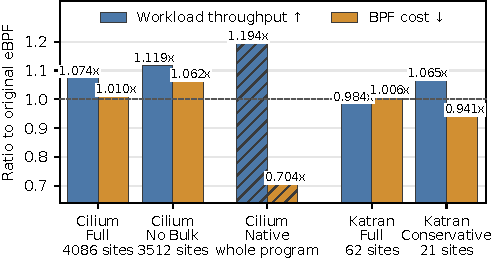
\includegraphics[width=\columnwidth]{figures/sec-6-rq3-cilium-katran.pdf}
  \caption{Application throughput and BPF cost under different \lang{} policies (\S\ref{subsec:policy_sensitivity}). The dashed line marks original eBPF, and the hatched bars replace whole Cilium programs with trusted native code (\S\ref{subsec:native_upper_bound}).}
  \label{fig:app_policy_probes}
\end{figure}



\subsection{RQ3: Sensitivity to Operation-Selection Policy}
\label{subsec:policy_sensitivity}


RQ3 evaluates how the choice of \lang operations affects these gains.
% RQ3 评估 \lang 操作的选择如何影响这些收益。
Which \lang operations to enable is a policy decision above \tool, and a performance one: each rewritten site trades the work that a shorter native sequence saves against its cost and its placement in a particular datapath.
% 启用哪些 \lang 操作是位于 \tool 之上的策略决定，也是性能决定：每个改写站点都要在更短的本地序列节省的工作与其代价及其在特定数据路径中的位置之间权衡。
A simple policy maximizes coverage, enabling every implemented operation and rewriting as many sites as possible.
% 一种简单的策略是最大化覆盖：启用所有已实现的操作，改写尽可能多的站点。
Figure~\ref{fig:app_policy_probes} tests this policy by changing it in two ways on Cilium and Katran.
% 图通过在 Cilium 和 Katran 上以两种方式改变该策略来检验它。



For Cilium, we start from the full x86-64 policy used in RQ2, which rewrites 4086 sites, improves throughput to 1.074$\times$, and leaves BPF cost nearly unchanged at 1.010$\times$ (Figure~\ref{fig:app_policy_probes}).
% 对于 Cilium，我们从 RQ2 使用的完整 x86-64 策略出发：它改写 4086 个站点，吞吐量提高到 1.074 倍，BPF 成本几乎不变，为 1.010 倍。
Disabling only the bulk copy operation reduces the rewritten sites to 3512 but raises throughput further to 1.119$\times$.
% 只禁用批量拷贝操作后，改写站点减少到 3512 个，吞吐量却进一步提高到 1.119 倍。
BPF cost also rises, to 1.062$\times$, so the result does not mean that bulk copy is harmful in general.
% BPF 成本也上升到 1.062 倍，所以这一结果并不意味着批量拷贝总是有害。
Rather, an additional operation can increase the number of rewritten sites without improving the measured datapath: the saved instructions may not outweigh the overhead of the replacement, or they may not lie on the part of the datapath that dominates throughput.
% 它说明的是，多启用一个操作可以增加改写站点的数量，却不一定改善所测的数据路径：节省的指令可能抵不上替换的开销，或者不在决定吞吐量的那部分数据路径上。

Katran shows the same lesson more directly.
% Katran 更直接地体现了同样的结论。
The conservative ARM64 policy used in RQ2 rewrites 21 sites, improves throughput to 1.065$\times$, and reduces BPF cost to 0.941$\times$.
% RQ2 使用的保守 ARM64 策略改写 21 个站点，吞吐量提高到 1.065 倍，BPF 成本降到 0.941 倍。
A policy that enables every implemented ARM64 operation rewrites 62 sites, yet throughput falls to 0.984$\times$ and BPF cost rises to 1.006$\times$.
% 启用所有已实现 ARM64 操作的策略改写 62 个站点，但吞吐量降到 0.984 倍，BPF 成本升到 1.006 倍。
Because a single hot XDP path dominates Katran, this is a clear counterexample to maximizing coverage: more rewritten sites bring neither higher throughput nor lower BPF cost.
% 由于 Katran 由单条热 XDP 路径主导，这是最大化覆盖的一个清晰反例：改写更多站点既没有带来更高的吞吐量，也没有带来更低的 BPF 成本。

Together, the two cases show that the number of rewritten sites is the wrong objective for a \lang policy.
% 两个案例共同表明，改写站点的数量不是 \lang 策略的正确目标。
An operation should be enabled when its rewrites save enough work on the target workload to justify their cost.
% 只有当一个操作的改写在目标工作负载上节省的工作足以抵消其代价时，才应启用它。
We currently choose policies by an automatic search that enables each combination of operations, measures it on the workload, and keeps the best.
% 目前我们用自动搜索选择策略：启用每一种操作组合，在工作负载上测量，保留最好的一个。
The search is needed because the number of rewritten sites cannot predict how often each site runs or how rewrites interact.
% 之所以需要搜索，是因为改写站点的数量无法预测每个站点执行得多频繁，也无法预测多个改写之间如何相互影响。
Its cost, however, grows with the number of combinations, and it must be repeated for every workload and processor.
% 但搜索的代价随组合数量增长，而且必须对每个工作负载和处理器重复进行。
A cost model that combines program profiles with processor information could replace most of these measurements, which we leave to future work.
% 结合程序剖析和处理器信息的代价模型可以取代大部分这类测量，我们将其留作未来工作。


\subsection{RQ4: In-Kernel Native Upper Bound}
\label{subsec:native_upper_bound}

Unlike RQ1--RQ3, which evaluate \lang's operations, RQ4 uses \tool itself to replace whole Cilium programs with native code, placing \tool in a broader design space.
% 与评估 \lang 操作的 RQ1--RQ3 不同，RQ4 用 \tool 本身把整个 Cilium 程序替换为本地代码，把 \tool 放到更大的设计空间中考察。
In this experiment, each Cilium BPF program is compiled from the same C source along two paths: the proof sequence is the normal eBPF bytecode that the verifier checks, while the native code is the same source compiled with LLVM \texttt{-O2} directly to native code.
% 在这个实验中，每个 Cilium BPF 程序从同一份 C 源码沿两条路径编译：证明序列是验证器检查的普通 eBPF 字节码，本地代码是用 LLVM -O2 把同一源码直接编译成的本地代码。
The verifier still checks the eBPF proof sequence on every load, but the equivalence between the two compilations is trusted rather than proved, so the application's native code and the path that loads it become part of the TCB.
% 验证器仍在每次加载时检查 eBPF 证明序列，但两种编译结果之间的等价性是被信任的而非被证明的，因此应用的本地代码及加载它的路径成为 TCB 的一部分。
The 2.358$\times$ upper bound is not comparable to the characterization's 1.57$\times$ microbenchmark gap, which measures microbenchmarks in isolation rather than Cilium's full datapath.
% 2.358 倍的上界不能与特征分析中 1.57 倍的微基准差距直接比较，后者测的是孤立的微基准，而不是 Cilium 的完整数据路径。

We use Cilium for this upper-bound study because it is the same kind of datapath workload evaluated above.
% 我们用 Cilium 做这项上界研究，因为它与上文评估的是同类数据路径工作负载。
The in-kernel native experiment uses the same x86-64 KVM application setup as the Cilium \lang runs.
% 内核内本地执行实验使用与 Cilium \lang 运行相同的 x86-64 KVM 应用配置。
It is not a claim about Cilium control-plane throughput: it measures steady-state datapath throughput after endpoint setup, with runtime reload and regeneration controllers disabled and the Cilium agent paused during measured workload samples.
% 它并不涉及 Cilium 控制面的吞吐量：它测量端点建立之后的稳态数据路径吞吐量，测量期间关闭了运行时重载和重新生成控制器，并暂停了 Cilium agent。

Trusting the native code raises the performance ceiling considerably.
% 信任本地代码会大幅提高性能上限。
Cilium throughput improves by 2.358$\times$ over original eBPF, and BPF cost drops from 488.7~ns to 262.3~ns per run, 1.86$\times$ lower.
% Cilium 吞吐量相对原版 eBPF 提高到 2.358 倍，BPF 成本从每次运行 488.7 ns 降到 262.3 ns，降低到原来的 1/1.86。

The gain comes at the cost of a larger TCB.
% 这一收益的代价是更大的 TCB。
In the Cilium run, 113 programs are replaced with native code, and 22 programs that have no native version run as eBPF.
% 在 Cilium 运行中，113 个程序被替换为本地代码，22 个没有本地版本的程序仍以 eBPF 运行。
The native code comes from 8 object files.
% 这些本地代码来自 8 个目标文件。
These numbers do not measure the TCB in lines of code, but they show how much native code the kernel must trust.
% 这些数字并不是以代码行数衡量的 TCB，但它们显示了内核必须信任多少本地代码。

This places original eBPF, \tool with \lang, and in-kernel native execution at three points in the same design space.
% 这样，原版 eBPF、带 \lang 的 \tool 和内核内本地执行就是同一设计空间中的三个点。
Original eBPF is the most conservative: it trusts only the existing verifier and JIT but pays for the limited eBPF instruction set.
% 原版 eBPF 最保守：它只信任现有的验证器和 JIT，但要为有限的 eBPF 指令集付出代价。
In-kernel native execution is the fastest but trusts the native code of whole programs and the path that loads it.
% 内核内本地执行最快，但要信任整个程序的本地代码以及加载它的路径。
\lang lies in between: its 1.074$\times$ Cilium throughput gain recovers 5.4\% of the gap to the 2.358$\times$ upper bound $((1.074{-}1)/(2.358{-}1))$, compared with 42\% on the microbenchmarks, because real datapaths spend most of their time in helpers, maps, and tail calls that \lang does not target.
% \lang 介于两者之间：它在 Cilium 上 1.074 倍的吞吐量提升追回了与 2.358 倍上界之间差距的 5.4\%，而在微基准上是 42\%，因为真实数据路径的大部分时间花在 \lang 不针对的辅助函数、map 和尾调用上。
\lang does not reach the upper bound, but it speeds up programs through a small set of kernel-defined operations rather than trusting the native code of whole programs.
% \lang 达不到上界，但它通过一小组由内核定义的操作来加速程序，而不必信任整个程序的本地代码。
The added trust is correspondingly small.
% 相应地，增加的信任也很小。
Proving whole-program native code equivalent to its bytecode amounts to verifying an optimizing compiler's output for an entire program, which remains impractical, so whole-program replacement must trust that code without proof.
% 证明整个程序的本地代码与其字节码等价，相当于验证优化编译器对整个程序的输出，目前仍不现实，因此整程序替换只能在没有证明的情况下信任这些代码。
An operation's native code, in contrast, is one or two machine instructions, and two lemmas prove it equivalent to its proof sequence (\S\ref{sec:formal-verification}).
% 相比之下，一个操作的本地代码只有一两条机器指令，两个引理就能证明它与证明序列等价。
